\documentclass{MIPRO}

\usepackage{cite}
\usepackage{amsmath,amssymb,amsfonts}
\usepackage{algorithmic}
\usepackage{graphicx}
\usepackage{textcomp}
\usepackage{xcolor}
\usepackage[T1]{fontenc}
\usepackage[ancient]{flushend}
\usepackage{multirow}
\usepackage{multicol}
\usepackage{array}
\usepackage{url}

\begin{document}

\title{Instructions for Preparation of Papers for MIPRO 2023}

\author{
\IEEEauthorblockN{
A.B. Firstauthor\IEEEauthorrefmark{1},
C. Secondauthor\IEEEauthorrefmark{2},
D.E. Thirdauthor\IEEEauthorrefmark{3}
}

\IEEEauthorblockA{\IEEEauthorrefmark{1} %1st affiliation 
Name of Institution/Department, City, Country}

\IEEEauthorblockA{\IEEEauthorrefmark{2} %2nd affiliation 
Name of Institution/Department, City, Country}

e-mail@address

\thanks{Identify applicable sponsor/s here. If no sponsors, delete this Latex command}
}

\maketitle

\begin{abstract}
The abstract should outline the main ideas and results of the paper. It should not exceed 200 words. Do not cite references in the abstract. 
\end{abstract}

\renewcommand\IEEEkeywordsname{Keywords}
\begin{IEEEkeywords}
\textit{component, formatting, style, styling, insert (key words)}
\end{IEEEkeywords}

\section{INTRODUCTION}

These instructions give you guidelines for typing camera‑ready papers for the 45\textsuperscript{th} Jubilee International Convention MIPRO 2023.

The latest version of this template can be found on GitHub at URL \url{https://github.com/sgros/mipro-template}. In case you have a problem, or or you want to contribute to this template, please use GitHub's issue tracker and pull requests.

The paper should consist of a title, author's name(s), affiliation, abstract, keywords, introduction, main text with section titles and subheadings (if any), conclusion, acknowledgment (if any), references and optional appendices. The length of the paper is limited to six pages including illustrations.

Your goal is to simulate the usual appearance of papers in an IEEE conference proceedings. The authors' affiliations should appear immediately following their names.

This electronic document is a “live” template and is used to format your paper and style the text. The template provides authors with most of the formatting specifications needed for preparing electronic versions of their papers. The various components of your paper (title, text, heads, etc.) are already defined on the style sheet, as illustrated by the portions given in this document. All margins (top and bottom margin of 25 mm, and left and right margin of 20 mm), column widths (of 82mm with the space between the two columns of 6mm), line spaces, and text fonts are prescribed; please do not alter them.

\subsection{Full-Sized Camera-Ready (CR) Copy}

Times New Roman font are strictly required. Follow the type sizes specified in Table \ref{type_sizes} (expressed in points). There are 72 points per inch, and 1 point is about 0.35 mm.

\begin{table}[h]
%\renewcommand{\arraystretch}{1.3}
\caption{Type Size for Camera-Ready Papers}
\label{type_sizes}
\centering
\begin{tabular}{|c|p{10em}|c|c|} 
 \hline
 \multirow{2}{*}{Type size} & \multicolumn{3}{|c|}{Appearance} \\
 \cline{2-4}
 & Regular & Bold & Italic \\
 \hline\hline
 8 & Section titles, references, tables, table names, first letters in table captions, figure captions, footnotes, text subscripts and superscripts &  &  \\ 
 \hline
 9 &  & Abstract,keywords & \\
 \hline
 10 & Authors’ affiliations, main text, equations, first letters in section titles & & Subheading \\
 \hline
 11 & Author's names & & \\
 \hline
 24 & Paper title & & \\ 
 \hline
\end{tabular}
\end{table}

Prepare your camera‑ready paper on the A4 paper size (210 mm x 297 mm). You are not allowed to use US letter-sized paper.

Justify both left and right columns. On the last page of your paper, adjust the lengths of the columns so that they are equal. Use automatic hyphenation and check spelling. Do not add page numbers.

\section{HELPFUL HINTS}

\subsection{Abbreviations and Acronyms}

Define abbreviations and acronyms the first time they are used in the text, even after they have been defined in the abstract. Abbreviations such as IEEE, SI, MKS, CGS, sc, dc, and rms do not have to be defined. Do not use abbreviations in the title or heads unless they are unavoidable.

\subsection{Units}

\begin{itemize}
    \item Use either SI (MKS) or CGS as primary units. (SI units are encouraged.) An exception would be the use of English units as identifiers in trade, such as “3.5-inch disk drive”.
    \item Avoid combining SI and CGS units, such as current in amperes and magnetic field in oersteds. This often leads to confusion because equations do not balance dimensionally. If you must use mixed units, clearly state the units for each quantity that you use in an equation.
    \item Do not mix complete spellings and abbreviations of units: “Wb/m2” or “webers per square meter”, not “webers/m2”. Spell out units when they appear in text: “. . . a few henries”, not “. . . a few H”.
    \item Use a zero before decimal points: “0.25”, not “.25”. Use “cm3”, not “cc”. 
\end{itemize}

\subsection{Figures and Tables}

Place figures and tables at the top and bottom of columns. Avoid placing them in the middle of columns. Large figures and tables may span across both columns. Figure captions should be below the figures; table heads should appear above the tables. Insert figures and tables after they are cited in the text. Use the abbreviation “Fig. 1”, even at the beginning of a sentence.

\begin{figure}
  \label{fig:figure1}
  \centering
  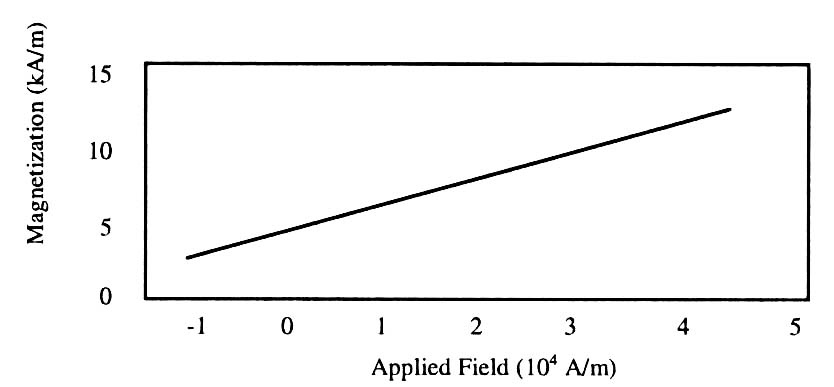
\includegraphics{figure1.jpg}
  \caption{Magnetization as a function of applied field. Note how the caption is centered in the column}
\end{figure}

Use words rather than symbols or abbreviations when writing Figure axis labels to avoid confusing the reader. As an example, write the quantity “Magnetization”, or “Magnetization, M”, not just “M”. If including units in the label, present them within parentheses. Do not label axes only with units. In the example, write “Magnetization (A/m)” or “Magnetization {A[m(1)]}”, not just “A/m”. Do not label axes with a ratio of quantities and units. For example, write “Temperature (K)”, not “Temperature/K”.

\subsection{Equations}

Number equations consecutively. Equation numbers, within parentheses, are to position flush right, as in (1), using a right tab stop. To make your equations more compact, you may use the solidus ( / ), the exp function, or appropriate exponents. Italicize Roman symbols for quantities and variables, but not Greek symbols. Use a long dash rather than a hyphen for a minus sign. Punctuate equations with commas or periods when they are part of a sentence, as in

\begin{equation}
    \alpha + \beta = \chi
\end{equation}

Note that the equation is centered using a center tab stop. Be sure that the symbols in your equation have been defined before or immediately following the equation. Use “(1)”, not “Eq. (1)” or “equation (1)”, except at the beginning of a sentence: “Equation (1) is . . .”

\subsection{Some Common Mistakes}

\begin{itemize}
    \item The word “data” is plural, not singular.
    \item The subscript for the permeability of vacuum $\epsilon_0$, and other common scientific constants, is zero with subscript formatting, not a lowercase letter “o”.
    \item In American English, commas, semi-/colons, periods, question and exclamation marks are located within quotation marks only when a complete thought or name is cited, such as a title or full quotation. When quotation marks are used, instead of a bold or italic typeface, to highlight a word or phrase, punctuation should appear outside of the quotation marks. A parenthetical phrase or statement at the end of a sentence is punctuated outside of the closing parenthesis (like this). (A parenthetical sentence is punctuated within the parentheses.)
    \item A graph within a graph is an “inset”, not an “insert”. The word alternatively is preferred to the word “alternately” (unless you really mean something that alternates).
    \item Do not use the word “essentially” to mean “approximately” or “effectively”.
    \item In your paper title, if the words “that uses” can accurately replace the word “using”, capitalize the “u”; if not, keep using lower-cased.
    \item Be aware of the different meanings of the homophones “affect” and “effect”, “complement” and “compliment”, “discreet” and “discrete”, “principal” and “principle”.
    \item Do not confuse “imply” and “infer”.
    \item The prefix “non” is not a word; it should be joined to the word it modifies, usually without a hyphen.
    \item There is no period after the “et” in the Latin abbreviation “et al.”.
    \item The abbreviation “i.e.” means “that is”, and the abbreviation “e.g.” means “for example”.
\end{itemize}

An excellent style manual for science writers is \cite{young2002technical}.

If your native language is not English, try to get a native English‑speaking colleague, or somebody fluent in English to proofread your paper. Use grammar existent in text editor.

\subsection{References}

The template will number citations consecutively within brackets \cite{eason1955certain}. The sentence punctuation follows the bracket \cite{maxwell1873treatise}. Refer simply to the reference number, as in \cite{jacobs1963fine}—do not use “Ref. \cite{jacobs1963fine}” or “reference \cite{jacobs1963fine}” except at the beginning of a sentence: “Reference \cite{jacobs1963fine} was the first . . .”

Number footnotes separately in superscripts. Place the actual footnote at the bottom of the column in which it was cited. Do not put footnotes in the reference list. Use letters for table footnotes.

Unless there are six authors or more give all authors' names; do not use “et al.”. Papers that have not been published, even if they have been submitted for publication, should be cited as “unpublished” \cite{elissa}. Papers that have been accepted for publication should be cited as “in press” \cite{nicole}. Capitalize only the first word in a paper title, except for proper nouns and element symbols.

For papers published in translation journals, please give the English citation first, followed by the original foreign-language citation \cite{yorozu1987electron}.

\subsection{Other Recommendations}

The Roman numerals are used to number the section headings. Do not number ACKNOWLEDGMENTS and REFERENCES, and begin Subheadings with letters. Use two spaces after periods (full stops). Hyphenate complex modifiers: “zero-field-cooled magnetization.” Avoid dangling participles, such as, “Using (1), the potential was calculated.” Write instead, “The potential was calculated using (1),” or “Using (1), we calculated the potential.”

\section{Conclusion}
Be brief and give most important conclusion from your paper. Do not use equations and figures here.

\section*{acknowledgment}

The preferred spelling of the word “acknowledgment” in America is without an “e” after the “g”. Avoid the stilted expression, “One of us (R. B. G.) thanks . . .”  Instead, try “R. B. G. thanks”. 

\bibliographystyle{IEEEtran}
\bibliography{references}

\end{document}
